%% =======================================================
%% Actividad 19: Práctica guiada con datos simulados
%%
%% Compilar desde actividades/: ./compilar.sh act19
%% Las figuras de img/ se generan con: python act19.py
%% =======================================================

%% ---- CONFIGURACIÓN ------------------------

\documentclass[11pt,letterpaper]{article}

\usepackage[indice]{tecnm}
\usepackage[T1]{fontenc}
\usepackage{amsmath}
\usepackage{xcolor}
\usepackage[most]{tcolorbox} % Carga tcolorbox con soporte para listings y saltos de página
\tcbuselibrary{listings, skins, breakable}
\setlength{\emergencystretch}{3em} % Evita líneas desbordadas por palabras en \texttt

% Paleta de colores (estilo GitHub Light / VS Code)
\definecolor{codebg}{HTML}{F8F9FA}       % Fondo del código
\definecolor{codehead}{HTML}{E9ECEF}     % Fondo de la barra de título
\definecolor{codeborder}{HTML}{CED4DA}   % Borde de la tarjeta
\definecolor{codetitle}{HTML}{212529}    % Texto del título
\definecolor{codekw}{HTML}{0550AE}       % Palabras clave (import, def, for...)
\definecolor{codefunc}{HTML}{8250DF}     % Funciones y métodos (describe, groupby...)
\definecolor{codestr}{HTML}{0A3069}      % Strings
\definecolor{codecomm}{HTML}{6E7781}     % Comentarios
\definecolor{codenum}{HTML}{8C959F}      % Números de línea
\definecolor{codeid}{HTML}{24292F}       % Texto general

% Configuración base de listings
\lstdefinestyle{pythonestilo}{
  language=Python,
  basicstyle=\ttfamily\footnotesize\color{codeid},
  keywordstyle=\color{codekw}\bfseries,
  keywordstyle=[2]\color{codefunc}, % Estilo secundario para métodos de datos
  stringstyle=\color{teal!80!black},
  commentstyle=\color{codecomm}\itshape,
  morekeywords={as, True, False, None, with, yield, lambda},
  morekeywords=[2]{shapiro, levene, ttest_ind, mannwhitneyu, confidence_interval, describe, boxplot, default_rng, normal, load_iris, mean, sqrt, concatenate, print, len, sum, max, DataFrame, Series, value_counts, reindex, mean, std, var, randint, normal, seed, cumsum, poisson, binom, pmf, norm, fit, kde, bincount, linspace, train_test_split, make_blobs, GaussianNB, chisquare, pdf, cdf, hist, bar, plot, axhline, axvline, fill_between, subplots, figure, concat, nunique, load_iris, diff, sort, unique},
  numbers=left,
  numberstyle=\tiny\ttfamily\color{codenum},
  stepnumber=1,
  numbersep=10pt,
  showstringspaces=false,
  morestring=[b]{"""},
  tabsize=4,
  breaklines=true,
  breakatwhitespace=true,
  columns=flexible,
  keepspaces=true,
  literate=
    {á}{{\'a}}1 {é}{{\'e}}1 {í}{{\'i}}1 {ó}{{\'o}}1 {ú}{{\'u}}1
    {Á}{{\'A}}1 {É}{{\'E}}1 {Í}{{\'I}}1 {Ó}{{\'O}}1 {Ú}{{\'U}}1
    {ñ}{{\~n}}1 {Ñ}{{\~N}}1 {¿}{{?`}}1 {¡}{{!`}}1 {°}{{$^\circ$}}1
}

% Definición del entorno personalizado \begin{codigo}{Título}{etiqueta}
% \newtcblisting[auto counter, number within=section]{codigo}[2][]{
\newtcblisting[auto counter]{codigo}[2][]{
  listing only,
  breakable,                    % Permite que el bloque se divida si pasa de página
  enhanced,
  colback=codebg,
  colframe=codeborder,
  colbacktitle=codehead,
  coltitle=codetitle,
  fonttitle=\bfseries\small\sffamily,
  boxrule=0.6pt,
  arc=4pt,                      % Bordes redondeados
  left=20pt,                    % Espacio izquierdo para los números de línea
  right=8pt,
  top=6pt,
  bottom=6pt,
  toptitle=4pt,
  bottomtitle=4pt,
  before skip=12pt,
  after skip=12pt,
  listing options={style=pythonestilo},
  title={Código \thetcbcounter: #2},
  #1
}

% Paleta para salida de consola (estilo terminal limpia)
\definecolor{termbg}{HTML}{212529}      % Fondo oscuro tipo terminal
\definecolor{termhead}{HTML}{343A40}    % Barra superior
\definecolor{termtext}{HTML}{F8F9FA}    % Texto claro de alta legibilidad
\definecolor{termborder}{HTML}{495057}  % Borde

% Entorno \begin{consola}[label=out:iris]{Título}
\newtcblisting[auto counter]{consola}[2][]{
  listing only,
  breakable,
  colback=termbg,
  colframe=termborder,
  colbacktitle=termhead,
  coltitle=termtext,
  colupper=termtext,
  fonttitle=\bfseries\small\sffamily,
  boxrule=0.6pt,
  arc=4pt,
  left=8pt,
  right=8pt,
  top=6pt,
  bottom=6pt,
  toptitle=4pt,
  bottomtitle=4pt,
  before skip=12pt,
  after skip=12pt,
  listing options={
    basicstyle=\ttfamily\scriptsize\color{termtext}, % \scriptsize evita que las tablas de Pandas se partan de línea
    breaklines=true,
    columns=fixed,        % Mantiene alineadas las columnas de Pandas
    keepspaces=true,
    showstringspaces=false,
    literate=
      {á}{{\'a}}1 {é}{{\'e}}1 {í}{{\'i}}1 {ó}{{\'o}}1 {ú}{{\'u}}1
      {Á}{{\'A}}1 {É}{{\'E}}1 {Í}{{\'I}}1 {Ó}{{\'O}}1 {Ú}{{\'U}}1
      {ñ}{{\~n}}1 {Ñ}{{\~N}}1 {°}{{$^\circ$}}1
  },
  title={Salida \thetcbcounter: #2},
  #1
}

%% ---- DATOS DE LA MATERIA ------------------------

\materia{Modelos Estadísticos para el Aprendizaje \\ Automático y Ciencia de Datos}
\actividad{Tema 3.1 Conceptos de las Pruebas de Hipótesis \\ Actividad 19 - Práctica guiada con datos simulados}

\profesor{Dr. José Ismael Ojeda Campaña}
%\fecha{15 de octubre de 2026}    % opcional; por defecto es la fecha de hoy

\begin{document}
\portada
\indicegeneral

%% ---- CONTENIDO ---------------------------------

\section{Introducción}

Las actividades anteriores definieron los componentes de una prueba de hipótesis. En esta se aplican a un conjunto de datos: se compara una variable entre dos grupos con una prueba paramétrica (la $t$ de Student) y con una no paramétrica (Mann-Whitney), y se interpreta el resultado con el valor $p$, la decisión sobre $H_0$ y el riesgo de cometer un error tipo I o tipo II \parencite{tecnm2026_documento_fuente}.

El flujo de trabajo es el que recomienda el documento fuente: primero se revisa si los datos cumplen las condiciones de las pruebas paramétricas (normalidad y varianzas iguales) y, según eso, se elige la prueba \parencite{tecnm2026_documento_fuente}. Además, como en un conjunto de datos real nunca se sabe si se cometió un error, se simulan datos con realidad conocida para estimar las probabilidades de los dos errores.

\section{Marco conceptual}

\subsection{Prueba t de Student y Mann-Whitney}

La $t$ de Student compara las medias de dos grupos y es una prueba paramétrica: requiere datos numéricos continuos con distribución normal y varianzas iguales entre los grupos. Mann-Whitney $U$ es su alternativa no paramétrica para dos grupos independientes, y se usa cuando los datos no son normales y la muestra es pequeña, o cuando son ordinales \parencite{tecnm2026_documento_fuente}. Cuando se cumplen los supuestos, ambas pruebas deben llegar a la misma decisión, y ese acuerdo da confianza en el resultado.

\subsection{Decisión y errores}

La regla de decisión compara el valor $p$ con el nivel de significancia $\alpha$: si $p \le \alpha$ se rechaza $H_0$ y si $p > \alpha$ no se rechaza. El error tipo I es rechazar $H_0$ siendo verdadera, con probabilidad máxima $\alpha$, y el error tipo II es no rechazarla siendo falsa, con probabilidad $\beta$ \parencite{tecnm2026_documento_fuente}. Un error tipo I solo puede ocurrir cuando se rechaza $H_0$ y uno tipo II solo cuando no se rechaza.

\section{Descripción de la actividad}

\textbf{Objetivo:} Aplicar los conceptos teóricos mediante el uso de datos reales o simulados \parencite{tecnm2026_documento_fuente}.

La actividad consta de cuatro tareas:

\begin{description}
    \item[1) Datos.] Cargar un conjunto de datos pequeño y explorarlo.
    \item[2) Supuestos.] Verificar si los datos cumplen las condiciones de la prueba paramétrica.
    \item[3) Prueba de hipótesis.] Aplicar la prueba $t$ de Student y la de Mann-Whitney, y decidir sobre $H_0$.
    \item[4) Riesgo de error.] Interpretar el valor $p$ y estimar con simulación el riesgo de error tipo I y tipo II.
\end{description}

\section{Desarrollo}

Las tareas se resolvieron en el script que utiliza \texttt{numpy}, \texttt{pandas}, \texttt{scipy}, \texttt{scikit-learn} y \texttt{matplotlib}. Las figuras se guardan como imágenes PNG en la carpeta \texttt{img/}. El Código~\ref{cod:comun} contiene las importaciones, las constantes ($\alpha = 0.05$ y la semilla del generador aleatorio) y la función auxiliar \texttt{guardar()}, que además muestra las figuras en pantalla cuando el código se ejecuta en un cuaderno. El cuaderno interactivo puede consultarse en Google Colab:

\begin{center}
    \url{https://colab.research.google.com/drive/1Vzf_81ySQ8TdV4dJuVaZzct0bmJYXDGK?usp=sharing}
\end{center}

\begin{codigo}[label=cod:comun]{Importaciones y función auxiliar}
import os

import matplotlib

# En Colab o Jupyter no existe __file__; ahí las figuras también se muestran en pantalla
EN_NOTEBOOK = '__file__' not in globals()
if not EN_NOTEBOOK:
    matplotlib.use('Agg')  # Como script, genera las figuras como archivos PNG sin abrir ventanas

import matplotlib.pyplot as plt
import numpy as np
import pandas as pd
from scipy import stats
from sklearn.datasets import load_iris

pd.set_option('display.width', 120)
SEMILLA = 42
ALFA = 0.05

# Carpeta donde se guardan las figuras que se incluyen en el reporte
BASE = os.getcwd() if EN_NOTEBOOK else os.path.dirname(os.path.abspath(__file__))
CARPETA_IMG = os.path.join(BASE, 'img')
os.makedirs(CARPETA_IMG, exist_ok=True)


def guardar(nombre):
    """Guarda la figura actual en la carpeta img/ y la muestra si se ejecuta en un notebook."""
    plt.tight_layout()
    plt.savefig(os.path.join(CARPETA_IMG, nombre), dpi=150)
    if EN_NOTEBOOK:
        plt.show()
    plt.close()
\end{codigo}

\subsection{Tarea 1: Datos y exploración}

Se usó el conjunto Iris, incluido en \texttt{scikit-learn}, que tiene 150 flores de tres especies con 50 flores por especie. La pregunta es si el ancho del sépalo es distinto entre \textit{Iris versicolor} e \textit{Iris virginica}. Las hipótesis son $H_0\colon \mu_{versicolor} = \mu_{virginica}$ y $H_1\colon \mu_{versicolor} \ne \mu_{virginica}$ (prueba bilateral), con $\alpha = 0.05$ fijado antes de calcular nada (Código~\ref{cod:t1}).

\begin{codigo}[label=cod:t1]{Tarea 1: exploración de los datos}
# Conjunto Iris (150 flores, incluido en scikit-learn). Pregunta: ¿el ancho del sépalo
# es distinto en Iris versicolor y en Iris virginica? (50 flores por especie).
iris = load_iris(as_frame=True)
df = iris.frame
df['especie'] = df['target'].map(dict(enumerate(iris.target_names)))
ancho = 'sepal width (cm)'
versicolor = df.loc[df['especie'] == 'versicolor', ancho].to_numpy()
virginica = df.loc[df['especie'] == 'virginica', ancho].to_numpy()

print("=== Tarea 1: exploración de los datos ===")
resumen = pd.DataFrame({
    'versicolor': pd.Series(versicolor).describe(),
    'virginica': pd.Series(virginica).describe(),
}).loc[['count', 'mean', 'std', 'min', '50%', 'max']].round(3)
print(resumen)

fig, ejes = plt.subplots(1, 2, figsize=(10, 4))
ejes[0].boxplot([versicolor, virginica], tick_labels=['versicolor', 'virginica'])
ejes[0].set_ylabel('Ancho del sépalo (cm)')
ejes[0].set_title('Diagrama de caja')
for datos, color, nombre in [(versicolor, 'tab:blue', 'versicolor'), (virginica, 'tab:orange', 'virginica')]:
    ejes[1].hist(datos, bins=np.arange(2.0, 3.9, 0.2), alpha=0.6, color=color, label=nombre)
ejes[1].set_xlabel('Ancho del sépalo (cm)')
ejes[1].set_ylabel('Frecuencia')
ejes[1].set_title('Histogramas')
ejes[1].legend()
guardar('exploracion.png')
\end{codigo}

\begin{consola}[label=out:t1]{Ejecución de \texttt{act19.py}: Tarea 1}
=== Tarea 1: exploración de los datos ===
       versicolor  virginica
count      50.000     50.000
mean        2.770      2.974
std         0.314      0.322
min         2.000      2.200
50%         2.800      3.000
max         3.400      3.800
\end{consola}

Cada grupo tiene 50 flores. La media de \textit{versicolor} es 2.770~cm y la de \textit{virginica} es 2.974~cm, una diferencia de 0.204~cm, con desviaciones estándar parecidas (0.314 y 0.322). La Figura~\ref{fig:expl} muestra que las distribuciones se solapan bastante, aunque \textit{virginica} está desplazada hacia valores mayores.

\begin{figure}[htbp]
\centering
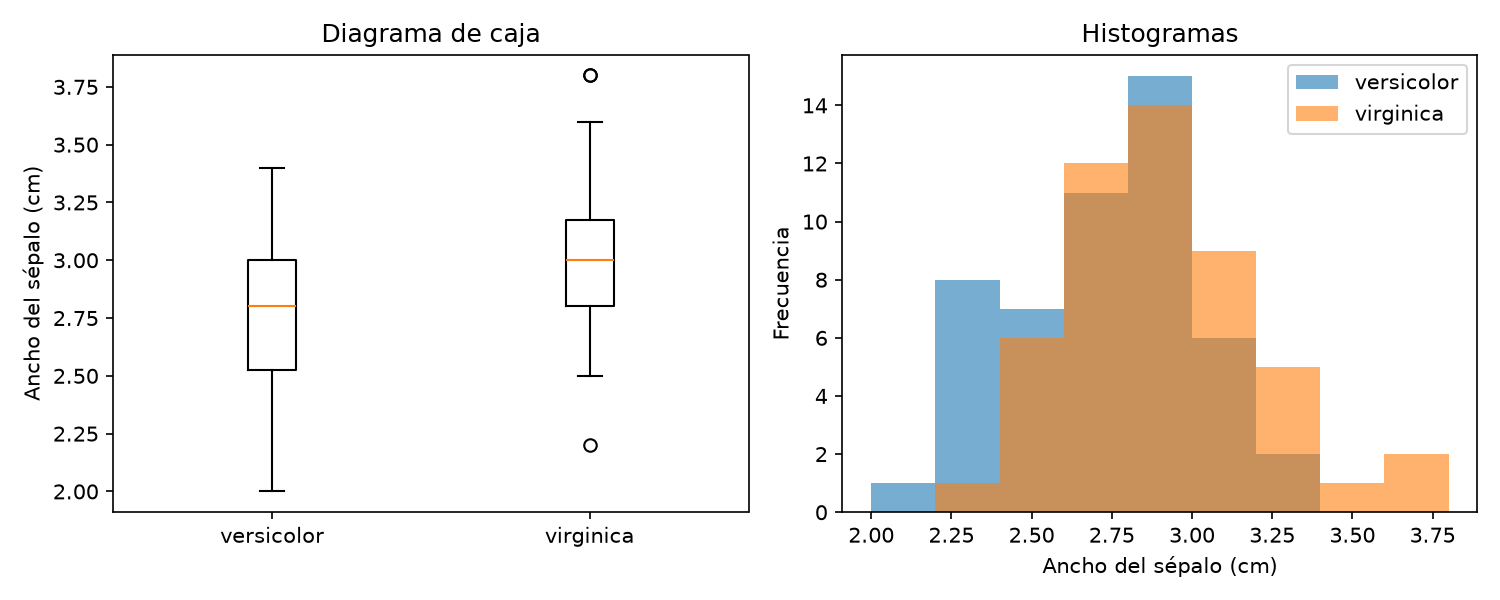
\includegraphics[width=\textwidth]{img/exploracion.png}
\caption{Ancho del sépalo por especie: diagrama de caja e histogramas.}
\label{fig:expl}
\end{figure}

\subsection{Tarea 2: Verificación de supuestos}

La $t$ de Student clásica requiere normalidad en cada grupo y varianzas iguales. Se comprobaron con la prueba de Shapiro-Wilk, cuya hipótesis nula es que los datos son normales, y con la de Levene, cuya hipótesis nula es que las varianzas son iguales (Código~\ref{cod:t2}).

\begin{codigo}[label=cod:t2]{Tarea 2: verificación de supuestos}
# La t de Student pide normalidad en cada grupo (Shapiro-Wilk) y, en su versión clásica,
# varianzas iguales (Levene). Si no se cumplen, se usa Mann-Whitney.
print("\n=== Tarea 2: supuestos ===")
for nombre, datos in [('versicolor', versicolor), ('virginica', virginica)]:
    w, p = stats.shapiro(datos)
    print(f"Shapiro-Wilk {nombre}: W = {w:.4f}, p = {p:.4f}")
estad_lev, p_lev = stats.levene(versicolor, virginica)
print(f"Levene (varianzas iguales): estadístico = {estad_lev:.4f}, p = {p_lev:.4f}")
\end{codigo}

\begin{consola}[label=out:t2]{Ejecución de \texttt{act19.py}: Tarea 2}
=== Tarea 2: supuestos ===
Shapiro-Wilk versicolor: W = 0.9741, p = 0.3380
Shapiro-Wilk virginica: W = 0.9674, p = 0.1809
Levene (varianzas iguales): estadístico = 0.0873, p = 0.7683
\end{consola}

En ambas especies el valor $p$ de Shapiro-Wilk es mayor que 0.05 (0.338 y 0.181), así que no se rechaza la normalidad. En Levene, $p = 0.768$, así que no se rechaza la igualdad de varianzas. Los supuestos se cumplen y la $t$ de Student es apropiada. Se aplica también Mann-Whitney para comprobar que la conclusión no depende de la prueba elegida.

\subsection{Tarea 3: Pruebas de hipótesis}

El Código~\ref{cod:t3} calcula la $t$ de Student, el intervalo de confianza del 95\,\% de la diferencia, la $d$ de Cohen (diferencia de medias en unidades de desviación estándar) y la prueba de Mann-Whitney. Como los grupos tienen el mismo tamaño y varianzas similares, la $t$ de Welch, que no supone varianzas iguales, da el mismo resultado.

\begin{codigo}[label=cod:t3]{Tarea 3: pruebas de hipótesis}
# H0: mu_versicolor = mu_virginica     H1: mu_versicolor != mu_virginica (bilateral)
print(f"\n=== Tarea 3: pruebas de hipótesis (alfa = {ALFA}) ===")
dif = versicolor.mean() - virginica.mean()
gl_clasica = len(versicolor) + len(virginica) - 2
t_student = stats.ttest_ind(versicolor, virginica, equal_var=True)
t_welch = stats.ttest_ind(versicolor, virginica, equal_var=False)
ic = t_student.confidence_interval(0.95)
sp = np.sqrt((versicolor.var(ddof=1) + virginica.var(ddof=1)) / 2)  # desviación combinada (n iguales)
d_cohen = dif / sp
u = stats.mannwhitneyu(versicolor, virginica, alternative='two-sided')

print(f"Diferencia de medias (versicolor - virginica): {dif:.3f} cm")
print(f"t de Student:  t = {t_student.statistic:.4f}, gl = {gl_clasica}, p = {t_student.pvalue:.5f}")
print(f"IC 95% de la diferencia: [{ic.low:.3f}, {ic.high:.3f}] cm")
print(f"t de Welch:    t = {t_welch.statistic:.4f}, p = {t_welch.pvalue:.5f}")
print(f"d de Cohen = {d_cohen:.3f}")
print(f"Mann-Whitney:  U = {u.statistic:.1f}, p = {u.pvalue:.5f}")
for nombre, p in [('t de Student', t_student.pvalue), ('Mann-Whitney', u.pvalue)]:
    decision = 'se rechaza H0' if p <= ALFA else 'no se rechaza H0'
    print(f"{nombre}: p = {p:.5f} {'<=' if p <= ALFA else '>'} {ALFA} -> {decision}")
\end{codigo}

\begin{consola}[label=out:t3]{Ejecución de \texttt{act19.py}: Tarea 3}
=== Tarea 3: pruebas de hipótesis (alfa = 0.05) ===
Diferencia de medias (versicolor - virginica): -0.204 cm
t de Student:  t = -3.2058, gl = 98, p = 0.00182
IC 95% de la diferencia: [-0.330, -0.078] cm
t de Welch:    t = -3.2058, p = 0.00182
d de Cohen = -0.641
Mann-Whitney:  U = 841.0, p = 0.00457
t de Student: p = 0.00182 <= 0.05 -> se rechaza H0
Mann-Whitney: p = 0.00457 <= 0.05 -> se rechaza H0
\end{consola}

El estadístico de la $t$ de Student es $t = -3.206$ con 98 grados de libertad y $p = 0.00182$. Como $0.00182 \le 0.05$, se rechaza $H_0$. Mann-Whitney da $U = 841$ y $p = 0.00457$, también menor que 0.05, así que las dos pruebas coinciden. El signo negativo de $t$ solo indica que la media de \textit{versicolor} es menor.

\subsection{Tarea 4: Riesgo de error tipo I y tipo II}

En los datos reales no se sabe si $H_0$ es verdadera, así que no se puede saber si se cometió un error. Para estimar los riesgos se simularon 10\,000 experimentos con datos normales donde sí se conoce la realidad (Código~\ref{cod:t4}). Con $H_0$ verdadera (misma media en ambos grupos) la proporción de rechazos estima $\alpha$. Con $H_1$ verdadera, usando como diferencia real la observada (0.204~cm) y la desviación estándar combinada de los datos, la proporción de no rechazos estima $\beta$. Esto supone que la diferencia observada es la real, que es solo un escenario para la simulación.

\begin{codigo}[label=cod:t4]{Tarea 4: simulación de errores}
# Se repite la prueba 10 000 veces con datos simulados donde se conoce la realidad.
# Con H0 verdadera, la proporción de rechazos estima alfa (error tipo I).
# Con H1 verdadera (diferencia observada), la proporción de no rechazos estima beta.
print("\n=== Tarea 4: simulación de errores ===")
rng = np.random.default_rng(SEMILLA)
N_SIM = 10_000
media_comun = np.mean(np.concatenate([versicolor, virginica]))


def simular(n, diferencia):
    """Devuelve los valores p de N_SIM pruebas t con muestras normales de tamaño n."""
    g1 = rng.normal(media_comun - diferencia / 2, sp, size=(N_SIM, n))
    g2 = rng.normal(media_comun + diferencia / 2, sp, size=(N_SIM, n))
    return stats.ttest_ind(g1, g2, axis=1).pvalue


p_h0 = simular(50, 0.0)
filas = [('H0 verdadera', 50, 0.0, np.mean(p_h0 <= ALFA), 'error tipo I (alfa)')]
p_h1_50 = simular(50, abs(dif))
p_h1_10 = simular(10, abs(dif))
filas.append(('H1 verdadera', 50, abs(dif), np.mean(p_h1_50 > ALFA), 'error tipo II (beta)'))
filas.append(('H1 verdadera', 10, abs(dif), np.mean(p_h1_10 > ALFA), 'error tipo II (beta)'))
tabla = pd.DataFrame(filas, columns=['realidad', 'n por grupo', 'diferencia', 'proporción', 'estima'])
print(tabla.round(4).to_string(index=False))

fig, ejes = plt.subplots(1, 3, figsize=(12, 3.8), sharey=True)
for eje, p, titulo in [(ejes[0], p_h0, 'H0 verdadera, n = 50'),
                       (ejes[1], p_h1_50, 'H1 verdadera, n = 50'),
                       (ejes[2], p_h1_10, 'H1 verdadera, n = 10')]:
    eje.hist(p, bins=20, range=(0, 1), color='tab:gray', edgecolor='white')
    eje.axvline(ALFA, color='tab:red', linestyle='--', label=f'alfa = {ALFA}')
    eje.set_title(titulo)
    eje.set_xlabel('valor p')
ejes[0].set_ylabel('Frecuencia (de 10 000)')
ejes[0].legend()
guardar('simulacion_errores.png')
\end{codigo}

\begin{consola}[label=out:t4]{Ejecución de \texttt{act19.py}: Tarea 4}
=== Tarea 4: simulación de errores ===
    realidad  n por grupo  diferencia  proporción               estima
H0 verdadera           50       0.000      0.0459  error tipo I (alfa)
H1 verdadera           50       0.204      0.1166 error tipo II (beta)
H1 verdadera           10       0.204      0.7317 error tipo II (beta)
\end{consola}

\begin{figure}[htbp]
\centering
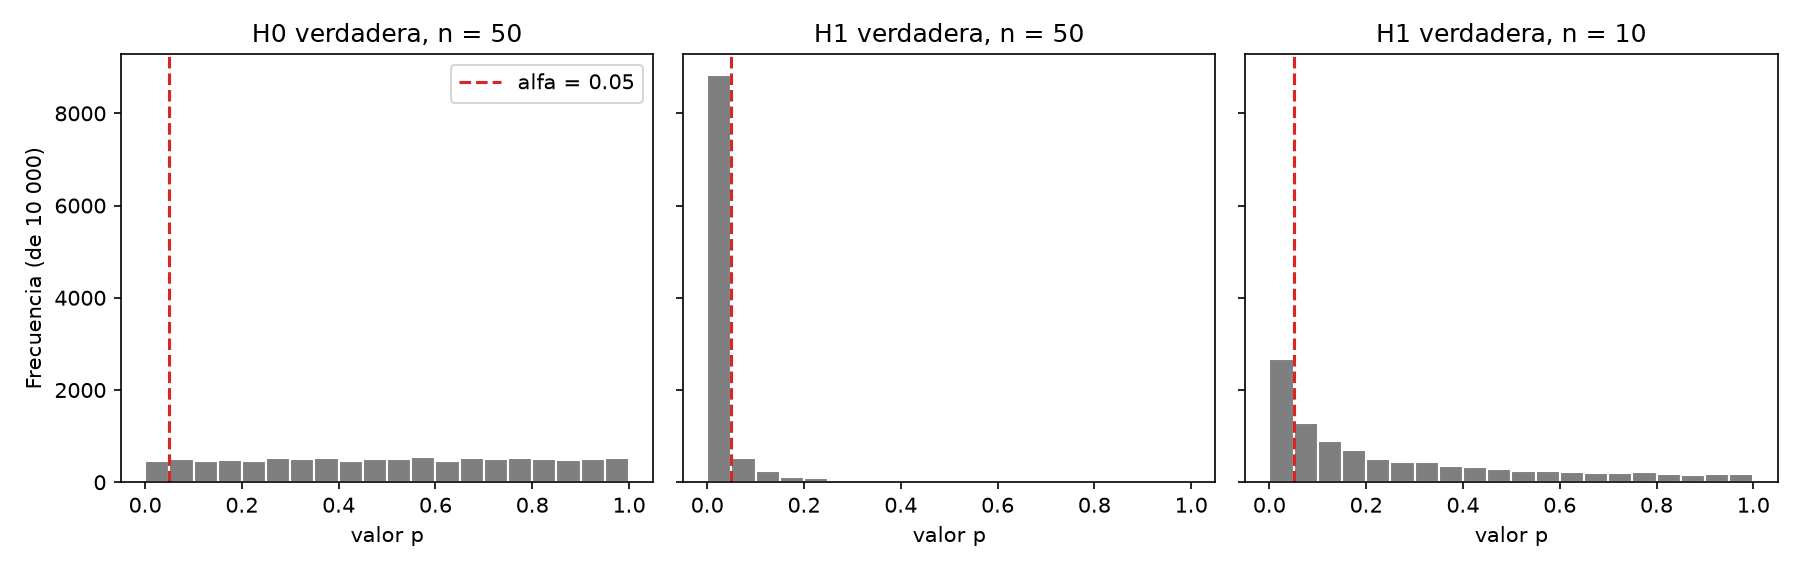
\includegraphics[width=\textwidth]{img/simulacion_errores.png}
\caption{Distribución del valor $p$ en 10\,000 simulaciones. Si $H_0$ es verdadera es uniforme y el 5\,\% queda a la izquierda de $\alpha$; si $H_1$ es verdadera se concentra cerca de 0, y menos con $n = 10$.}
\label{fig:sim}
\end{figure}

\section{Interpretación estadística}

\textbf{Valor $p$ y decisión.} La prueba $t$ dio $p = 0.0018$: si el ancho medio del sépalo fuera igual en las dos especies, una diferencia tan grande o mayor que 0.204~cm aparecería en menos del 0.2\,\% de las muestras. Como $p \le \alpha = 0.05$, se rechaza $H_0$ y se concluye que hay evidencia de que las medias son distintas; Mann-Whitney ($p = 0.0046$) llega a la misma decisión. El $p$ no es la probabilidad de que $H_0$ sea cierta. El intervalo de confianza del 95\,\% de la diferencia, $[-0.330, -0.078]$~cm, no contiene el 0, lo que concuerda con el rechazo, y muestra que la diferencia es pequeña: la $d$ de Cohen de 0.64 es un efecto de tamaño medio, con distribuciones muy solapadas.

\textbf{Riesgo de error tipo I.} Como se rechazó $H_0$, el único error posible en esta decisión es el tipo I, es decir, que las especies no difieran y que la diferencia haya sido casualidad. Su probabilidad máxima la fija $\alpha = 0.05$, y la simulación lo confirma: con $H_0$ verdadera se rechazó en 4.59\,\% de las 10\,000 pruebas, muy cerca de 5\,\%. Por tanto, aunque el $p$ observado es mucho menor que $\alpha$, el riesgo del procedimiento sigue siendo el $\alpha$ elegido. No se cometió un error tipo II porque ese error solo puede ocurrir cuando no se rechaza $H_0$.

\textbf{Riesgo de error tipo II.} Si no se hubiera rechazado $H_0$, el riesgo sería el error tipo II. La simulación estima que, si la diferencia real es 0.204~cm, con 50 flores por grupo $\beta = 0.117$ (la prueba detecta la diferencia en 88\,\% de los casos), pero con solo 10 flores por grupo $\beta$ sube a 0.732 y la diferencia pasaría inadvertida casi tres de cada cuatro veces. Esto confirma que aumentar el tamaño de la muestra es la forma de reducir $\beta$ sin tocar $\alpha$ \parencite{tecnm2026_documento_fuente}. Una limitación es que Iris es un conjunto clásico y no una muestra aleatoria de una población definida, por lo que el resultado ilustra el método más que una conclusión biológica.

\section{Conclusiones}

Con los datos de Iris se rechazó $H_0$ con la $t$ de Student ($t = -3.206$, $p = 0.0018$) y con Mann-Whitney ($p = 0.0046$): el ancho del sépalo de \textit{versicolor} es en promedio 0.204~cm menor que el de \textit{virginica}, con un efecto de tamaño medio ($d = 0.64$). Antes de elegir la prueba se verificaron la normalidad y la igualdad de varianzas, y que ambas pruebas coincidan refuerza la conclusión.

La simulación mostró los dos errores: con $H_0$ verdadera se rechazó 4.59\,\% de las veces, que corresponde a $\alpha$, y con una diferencia real de 0.204~cm el error tipo II fue de 0.117 con $n = 50$ y de 0.732 con $n = 10$. El valor $p$ resume la evidencia de una muestra, pero los riesgos de error dependen del diseño de la prueba, en particular de $\alpha$ y del tamaño de la muestra.

\referencias

\end{document}
